%
% homologieketten.tex
%
% (c) 2021 Prof Dr Andreas Müller, OST Ostschweizer Fachhochschule
%
\subsection{Homologie eines Kettenkomplexes
\label{buch:subsection:homologie-eines-kettenkomplexes}}
Wegzusammenhang lässt sich untersuchen, indem man in der Triangulation
nach Linearkombinationen von Kanten sucht, die als Rand die beiden Punkte
haben.
Zwei Punkte sind also nicht verbindbar und liegen damit in verschiedenen
Komponenten, wenn die beiden Punkte nicht Rand irgend einer
Linearkombination von Kanten sind.
Komponenten können also identifiziert werden, indem man unter allen
Linearkombinationen von Punkten, also $C_0$ all diejenigen ignoriert,
die Rand einer Linearkombinationv on Kanten sind, also $\partial_1C_1$.
Der Quotientenraum $H_0=C_0/\partial_1C_1$ enthält also für jede Komponente
eine Dimension.

Eine Dimension höher könnten wir danach fragen, ob sich ein geschlossener
Weg zusammenziehen lässt.
In der Triangulation zeichnet sich ein geschlossener Weg dadurch aus,
dass jedes Ende einer Kante auch Anfang einer Folgekante ist, dass also
der Rand der Linearkombination von Kanten 0 ist.
Algebraisch bedeutet dies, dass wir uns für diejenigen Linearkombinationen
$z\in C_1$ interessieren, die keinen Rand haben, für die also $\partial_1z=0$
gilt.

\begin{definition}
Die Elemente von
\[
Z_k
=
Z_k^C
=
\{z\in C_k\;|\; \partial_k z = 0\}
=
\ker \partial_k
\]
heissen die {\em ($k$-dimensionalen) Zyklen} von $C_*$.
\end{definition}

In einem Dreieck ist der Rand ein geschlossener Weg, der sich zusammenziehen
lässt, indem man ihn durch die Dreiecksfläche deformiert.
Entfernt man aber die Dreiecksfläche, ist diese Deformation nicht mehr
möglich.
Einen zusammenziehbaren Weg kann man sich also als den Rand eines Dreiecks
einer vorstellen.
``Löcher'' sind durch geschlossene Wege erkennbar, die nicht Rand eines
Dreiecks sein können.
Wir müssen also ``Ränder'' ignorieren.

\begin{definition}
Die Elemente von
\[
B_k
=
B_k^C
=
\{\partial_{k+1}z\;|\; C_{k+1}\}
=
\operatorname{im} \partial_{k+1}
\]
heissen die {\em ($k$-dimensionalen) Ränder} von $C_*$.
\end{definition}

Algebraisch ausgedrückt interessieren uns also nur Zyklen, die selbst
keine Ränder sind.
Der Quotientenraum $Z_1/B_1$ ignoriert unter den Zyklen diejenigen, die
Ränder sind, drückt also algebraisch die Idee des eindimensionalen
Zusammenhangs aus.
Wir definieren daher

\begin{definition}
Die $k$-dimensionale Homologiegruppe des Kettenkomplexes $C_*$ ist
\[
H_k(C) = Z_k/B_k = \ker \partial_k / \operatorname{im} \partial_{k+1}.
\]
Wenn nur von einem Kettenkomplex die Rede ist, kann auch $H_k(C)=H_k$
abgekürzt werden.
\end{definition}

% XXX Visualisierung Zyklen/Ränder, Klassen von Zyklen, die sich um einen
% XXX Rand unterscheiden

Die folgenden zwei ausführlichen Beispiele sollen zeigen, wie die
Homologiegruppe $H_2$ die Anwesenheit eines Hohlraumes detektieren kann,
der entsteht, wenn man aus einem Tetraeder das innere entfernt.

\begin{beispiel}
\begin{figure}
\centering
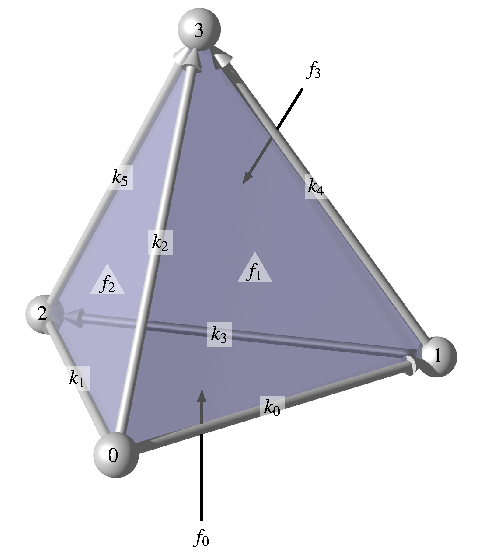
\includegraphics{chapters/95-homologie/images/tetraeder.pdf}
\caption{Triangulation eines Tetraeders, die Orientierung von Kanten
und Seitenflächen ist immer so gewählt, dass die Nummern der Ecken
aufsteigend sind.
\label{buch:homologie:tetraeder:fig}}
\end{figure}
Ein Tetraeder ist ein zweidmensionales Simplex, wir untersuchen seinen
Kettenkomplex und bestimmen die zugehörigen Homologiegruppen.
Zunächst müssen wir die einzelnen Mengen $C_k$ beschreiben und verwenden
dazu die Bezeichnungen gemäss Abbildung~\ref{buch:homologie:tetraeder:fig}.
$C_0$ ist der vierdimensionale Raum aufgespannt von den vier Ecken 
$0$, $1$, $2$ und $3$ des Tetraeders.
$C_1$ ist der sechsdimensionale Vektorraum der Kanten 
\[
k_0 = [0,1],\quad
k_1 = [0,2],\quad
k_2 = [0,3],\quad
k_3 = [1,2],\quad
k_4 = [1,3],\quad
k_5 = [2,3]
\]
Der Randoperator $\partial_1$ hat die Matrix
\[
\partial_1
=
\begin{pmatrix*}[r]
-1&-1&-1& 0& 0& 0\\
 1& 0& 0&-1&-1& 0\\
 0& 1& 0& 1& 0&-1\\
 0& 0& 1& 0& 1& 1
\end{pmatrix*}.
\]

Wir erwarten natürlich, dass sich zwei beliebige Ecken verbinden lassen,
dass es also nur eine Komponente gibt und dass damit $H_1=\Bbbk$ ist.
Dazu beachten wir, dass das Bild von $\partial_1$ genau aus den Vektoren
besteht, deren Komponentensumme $0$ ist.
Das Bild $B_0$ von $\partial_1$ ist daher die Lösungsmenge der einen
Gleichung
\(
x_0+x_1+x_2+x_3=0.
\)
Der Quotientenraum $H_0=Z_0/B_0 = C_0/\operatorname{im}\partial_1$
ist daher wie erwartet eindimensional.

Wir bestimmen jetzt die Homologiegruppe $H_1$.
Da sich im Tetraeder jeder geschlossene Weg zusammenziehen lässt,
erwarten wir $H_1=0$.

Die Menge der Zyklen $Z_1$ wird bestimmt, indem man die Lösungsmenge
des Gleichungssystems $\partial_1z=0$ bestimmt.
Der Gauss-Algorithmus für die Matrix $\partial_1$ liefert das
Schlusstableau
\[
\begin{tabular}{|>{$}c<{$}>{$}c<{$}>{$}c<{$}>{$}c<{$}>{$}c<{$}>{$}c<{$}|}
\hline
k_0&k_1&k_2&k_3&k_4&k_5\\
\hline
   1&  0&  0& -1& -1&  0\\
   0&  1&  0&  1&  0& -1\\
   0&  0&  1&  0&  1&  1\\
   0&  0&  0&  0&  0&  0\\
\hline
\end{tabular}
\]
Daraus lassen sich drei linear unabhängig eindimensionale Zyklen ablesen,
die zu den Lösungsvektoren
\[
z_1
=
\begin{pmatrix*}[r]
1\\
-1\\
0\\
1\\
0\\
0
\end{pmatrix*},
\qquad
z_2
=
\begin{pmatrix*}[r]
1\\
0\\
-1\\
0\\
1\\
0
\end{pmatrix*},
\qquad
z_3
=
\begin{pmatrix*}[r]
0\\
1\\
-1\\
0\\
0\\
1
\end{pmatrix*}
\]
gehören.

$C_2$ hat die vier Seitenflächen
\[
f_0=[0,1,2],\quad
f_1=[0,1,3],\quad
f_2=[0,2,3],\quad
f_3=[1,2,3]
\]
als Basis.
Der zweidimensionale Randoperator ist die $6\times 4$-Matrix 
\[
\partial_2
=
\begin{pmatrix*}[r]
 1& 1& 0& 0\\
-1& 0& 1& 0\\
 0&-1&-1& 0\\
 1& 0& 0& 1\\
 0& 1& 0&-1\\
 0& 0& 1& 1
\end{pmatrix*}.
\]
Man kann leicht nachrechnen, dass $\partial_1\partial_2=0$ ist, wie es
für einen Kettenkomplex sein muss.

Um nachzurechnen, dass die Homologiegruppe $H_1=0$ ist, müssen wir jetzt 
nachprüfen, ob jeder Zyklus in $Z_1$ auch Bild der Randabbildung $\partial_2$
ist.
Die ersten drei Spalten von $\partial_2$ sind genau die drei Zyklen
$z_1$, $z_2$ und $z_3$.
Insbesondere lassen sich alle Zyklen als Ränder darstellen, die
Homologiegruppe $H_1=0$ verschwindet.

Die Zyklen in $C_2$ sind die Lösungen von $\partial_2z=0$.
Der Gauss-Algorithmus für $\partial_2$ liefert das -Tableau
\[
\begin{tabular}{|>{$}c<{$}>{$}c<{$}>{$}c<{$}>{$}c<{$}|}
\hline
f_0&f_1&f_2&f_3\\
\hline
1&0&0& 1\\
0&1&0&-1\\
0&0&1& 1\\
0&0&0& 0\\
0&0&0& 0\\
0&0&0& 0\\
\hline
\end{tabular}
\]
Daraus liest man ab, dass es genau einen Zyklus nämlich
\[
z
=
\begin{pmatrix}
-1\\1\\-1\\1
\end{pmatrix}
\]
$Z_2$ besteht also aus Vielfachen des Vektors $z$.

Da es nur ein zweidimensionales Simplex gibt, ist $C_3$ eindimensional.
Die Randabbildung $\partial_3$ hat die Matrix
\[
\partial_3
=
\begin{pmatrix}
1\\
-1\\
1\\
-1
\end{pmatrix}.
\]
Die Zyklen $Z_2$ und die Ränder $B_2$ bilden also dieselbe Menge, auch
die Homologie-Gruppe $H_2$ ist $0$.

Da es keine vierdimensionalen Simplizes gibt, ist $B_3=0$.
Die Zyklen $Z_3$ bestehen aus den Lösungen von $\partial_3w=0$, da
aber $\partial_3$ injektiv ist, ist $Z_3=0$.
Daher ist auch $H_3=0$.
\end{beispiel}

\begin{beispiel}
Für dieses Beispiel entfernen wir das Innere des Tetraeders, es entsteht
ein Hohlraum.
Am Kettenkomplex der Triangulation ändert sich nur, dass $C_3$ jetzt 
nur noch den $0$-Vektor enthält.
Das Bild $B_2=\operatorname{im}\partial_3$ wird damit auch $0$-dimensional,
während es im vorigen Beispiel eindimensional war.
Die einzige Änderung ist also in der Homologiegruppe 
$H_2 = Z_2/B_2 = Z_2 / \{0\} \simeq \Bbbk$.
Die Homologiegruppe $H_2$ hat jetzt Dimension $1$ und zeigt damit den
Hohlraum an.
\end{beispiel}
